
\documentclass[aspectratio=169,14pt]{beamer}
\usetheme{default}\usecolortheme{default}\setbeamertemplate{navigation symbols}{}
\setbeamertemplate{footline}{\hfill{\scriptsize\color{covermuted}\insertframenumber/\inserttotalframenumber}\hspace{0.4cm}\vspace{0.15cm}}
\usepackage{fontspec}\usepackage{xeCJK}\setCJKmainfont{PingFang SC}[BoldFont=PingFang SC Semibold]\setmainfont{Helvetica Neue}[BoldFont=Helvetica Neue Bold]
\usepackage{xcolor}\usepackage{tikz}\usepackage{graphicx}\usepackage{fontawesome5}\usetikzlibrary{positioning,calc,arrows.meta,shadows}
\definecolor{bgmain}{RGB}{238,243,252}\definecolor{panel}{RGB}{238,244,255}\definecolor{factbg}{RGB}{246,242,235}\definecolor{coverprimary}{HTML}{2563EB}\definecolor{coveraccent}{HTML}{00A884}\definecolor{coverwarning}{HTML}{F59E0B}\definecolor{coverdark}{HTML}{1F2937}\definecolor{covermuted}{HTML}{64748B}\definecolor{titlecolor}{RGB}{30,30,30}\definecolor{muteddark}{RGB}{72,86,115}\definecolor{bluepanel}{RGB}{226,237,255}\definecolor{greenpanel}{RGB}{225,246,237}\definecolor{amberpanel}{RGB}{255,244,222}\definecolor{purplepanel}{RGB}{239,231,255}\setbeamercolor{background canvas}{bg=bgmain}
\newcommand{\plainbar}{\begin{tikzpicture}[remember picture, overlay]\fill[coverdark, opacity=0.07] (current page.south west) rectangle ([yshift=0.4cm]current page.south east);\draw[coveraccent, opacity=0.45, line width=0.8pt] ([yshift=0.4cm]current page.south west) -- ([yshift=0.4cm]current page.south east);\end{tikzpicture}}
\newcommand{\deckbackground}{\begin{tikzpicture}[remember picture, overlay]\fill[coverprimary!8] (current page.north west) rectangle (current page.south east);\fill[coverprimary!14] (current page.north west) ++(1.55,-1.35) circle (2.45cm);\fill[coveraccent!12] (current page.south east) ++(-1.9,1.45) circle (2.70cm);\fill[coverwarning!12] (current page.north east) ++(-2.9,-1.8) circle (0.85cm);\foreach \x in {-0.2,0.8,...,16.2} {\draw[coverprimary, opacity=0.045, line width=0.25pt] ([xshift=\x cm]current page.south west) -- ([xshift=\x cm]current page.north west);}\foreach \y in {-0.2,0.7,...,9.3} {\draw[coverprimary, opacity=0.04, line width=0.25pt] ([yshift=\y cm]current page.south west) -- ([yshift=\y cm]current page.south east);}\draw[coveraccent, opacity=0.38, line width=1.1pt] ([xshift=0.35cm,yshift=7.72cm]current page.south west) -- ++(3.25,0) -- ++(0.45,-0.45) -- ++(2.0,0);\draw[coverprimary, opacity=0.24, line width=1.0pt] ([xshift=9.35cm,yshift=8.25cm]current page.south west) -- ++(2.3,0) -- ++(0.55,-0.55) -- ++(3.2,0);\fill[coverdark, opacity=0.07] (current page.south west) rectangle ([yshift=0.42cm]current page.south east);\end{tikzpicture}}
\newcommand{\sectiontitle}[2]{\vspace{-0.52cm}\begin{center}{\fontsize{20}{24}\selectfont\bfseries\color{titlecolor} #1}\\[2pt]{\fontsize{9}{11}\selectfont\itshape\color{muteddark} #2}\end{center}\vspace{0.12cm}}
\newcommand{\portraitbox}[2]{\begin{tikzpicture}\node[draw=coverprimary!28, line width=0.7pt, fill=white, rounded corners=3pt, inner sep=2.5pt, drop shadow={shadow xshift=0.5pt, shadow yshift=-0.5pt, opacity=0.12}] {\includegraphics[width=2.4cm,height=2.9cm,keepaspectratio]{#1}};\end{tikzpicture}{\par\vspace{1pt}\fontsize{6.5}{7.5}\selectfont\color{covermuted} #2\par}}
\newcommand{\personslide}[9]{\begin{frame}\plainbar\vspace{-0.45cm}\begin{center}{\fontsize{22}{26}\selectfont\bfseries\color{coverdark} #1}\\[2pt]{\fontsize{9.5}{11.5}\selectfont\color{muteddark} #2}\end{center}\vspace{0.15cm}\begin{columns}[c]\begin{column}{0.22\textwidth}\centering #3\end{column}\begin{column}{0.28\textwidth}\begin{tikzpicture}\node[fill=greenpanel, rounded corners=4pt, inner xsep=6pt, inner ysep=5pt, text width=3.8cm, align=left] {{\fontsize{7}{8.5}\selectfont\bfseries\color{coveraccent!70!black} 获奖}\enspace{\fontsize{7}{8.5}\selectfont\color{coverdark!85} #4}\\[2.5pt]{\fontsize{7}{8.5}\selectfont\bfseries\color{coveraccent!70!black} 生卒}\enspace{\fontsize{7}{8.5}\selectfont\color{coverdark!85} #5}\\[2.5pt]{\fontsize{7}{8.5}\selectfont\bfseries\color{coveraccent!70!black} 身份}\enspace{\fontsize{7}{8.5}\selectfont\color{coverdark!85} #6}\\[2.5pt]{\fontsize{7}{8.5}\selectfont\bfseries\color{coveraccent!70!black} 机构}\enspace{\fontsize{7}{8.5}\selectfont\color{coverdark!85} #7}};\end{tikzpicture}\end{column}\begin{column}{0.48\textwidth}\begin{tikzpicture}\node[draw=coverprimary!35, fill=bluepanel, rounded corners=5pt, inner sep=7pt, text width=6.6cm, anchor=north west] at (0,0) {{\fontsize{8.6}{10.2}\selectfont\bfseries\color{coverprimary!82!black} 核心贡献}\\[3pt]{\fontsize{7.4}{9.2}\selectfont\color{coverdark!84} #8\\[3pt]\textbf{一句话：} #9}};\end{tikzpicture}\end{column}\end{columns}\end{frame}}

\begin{document}
\begin{frame}[plain]
\deckbackground
\begin{tikzpicture}[remember picture, overlay]
  \node[anchor=center, font=\fontsize{28}{34}\selectfont\bfseries, text=coverdark] at ([yshift=2.05cm]current page.center) {沃尔夫数学奖人物谱系};
  \node[anchor=center, font=\fontsize{15}{19}\selectfont, text=coverprimary!82!black] at ([yshift=0.86cm]current page.center) {第11集 \enspace·\enspace 动力系统与遍历理论};
  \node[anchor=center, font=\fontsize{12}{16}\selectfont\bfseries, text=coveraccent!76!black] at ([yshift=0.10cm]current page.center) {Dynamical Systems · Ergodic Theory · Rigidity};
  \draw[coveraccent, line width=1.4pt] ([yshift=-1.02cm, xshift=-4.55cm]current page.center) -- ([yshift=-1.02cm, xshift=4.55cm]current page.center);
  \node[anchor=center] at ([yshift=-1.90cm]current page.center) {\begin{tikzpicture}\node[rounded corners=8pt, fill=coverprimary!10, inner sep=4pt, minimum height=1.2em, font=\scriptsize\bfseries, text=coverprimary!85!black] at (-5.30,0) {Moser};\node[rounded corners=8pt, fill=coverprimary!10, inner sep=4pt, minimum height=1.2em, font=\scriptsize\bfseries, text=coverprimary!85!black] at (-2.65,0) {Arnold};\node[rounded corners=8pt, fill=coverprimary!10, inner sep=4pt, minimum height=1.2em, font=\scriptsize\bfseries, text=coverprimary!85!black] at (0.00,0) {Sinai};\node[rounded corners=8pt, fill=coverprimary!10, inner sep=4pt, minimum height=1.2em, font=\scriptsize\bfseries, text=coverprimary!85!black] at (2.65,0) {Furstenberg};\node[rounded corners=8pt, fill=coverprimary!10, inner sep=4pt, minimum height=1.2em, font=\scriptsize\bfseries, text=coverprimary!85!black] at (5.30,0) {Margulis};\end{tikzpicture}};
\end{tikzpicture}
\end{frame}
\begin{frame}
\plainbar
\sectiontitle{动力系统与遍历理论}{Dynamical Systems · Ergodic Theory · Rigidity}
\begin{center}\begin{tikzpicture}
  \node[draw=coverprimary!45, fill=bluepanel, rounded corners=5pt, inner sep=8pt, text width=11.2cm, align=left] at (0,1.05) {{\fontsize{8.3}{10}\selectfont\bfseries\color{coverprimary!80!black} 本集主线}\\[3pt]{\fontsize{7.4}{9.2}\selectfont\color{coverdark!84} 本集从 KAM 理论、经典力学和混沌讲到遍历理论、统计力学、测度刚性、Lie 群格和动力系统方法，展示“运动”如何变成结构理论。}};
  \node[draw=coverwarning!60, fill=amberpanel, rounded corners=5pt, inner sep=7pt, text width=11.2cm, align=center] at (0,-1.45) {{\fontsize{8.0}{9.8}\selectfont\bfseries\color{coverwarning!62!black} 开场问题}\\[-1pt]{\fontsize{7.4}{9}\selectfont\color{coverdark!82} 一个确定性系统为什么会表现得像随机？长期运动中哪些结构会保留下来？}};
\end{tikzpicture}\end{center}
\end{frame}
\begin{frame}
\plainbar
\sectiontitle{人物路线图}{从早期奠基到现代前沿}
\begin{center}
\begin{tikzpicture}[milestone/.style={draw=coverprimary!45, fill=panel, rounded corners=4pt, inner xsep=4.0pt, inner ysep=5pt, align=center, font=\fontsize{5.9}{7.2}\selectfont\bfseries}, arrow/.style={-{Stealth}, draw=coveraccent, line width=0.7pt}]
\node[milestone, fill=bluepanel] (m0) at (-5.50,1.0) {1994/95\\Moser\\KAM};
\node[milestone, fill=greenpanel] (m1) at (-2.75,1.0) {2001\\Arnold\\力学};
\node[milestone, fill=amberpanel] (m2) at (0.00,1.0) {1996/97\\Sinai\\遍历};
\node[milestone, fill=purplepanel] (m3) at (2.75,1.0) {2006/07\\Furstenberg\\边界};
\node[milestone, fill=bluepanel] (m4) at (5.50,1.0) {2005\\Margulis\\刚性};
\draw[arrow] (m0) -- (m1);
\draw[arrow] (m1) -- (m2);
\draw[arrow] (m2) -- (m3);
\draw[arrow] (m3) -- (m4);
  \node[draw=coverprimary!38, fill=white, rounded corners=5pt, inner sep=7pt, text width=11.4cm, align=left] at (0,-1.25) {{\fontsize{8.0}{9.8}\selectfont\bfseries\color{coverprimary!80!black} 叙事线}\\[-1pt]{\fontsize{7.2}{8.8}\selectfont\color{coverdark!82} 从 Moser 和 Arnold 的 KAM/力学传统，到 Sinai 的混沌与统计力学，再到 Furstenberg 和 Margulis 的遍历、刚性与数论应用，本集展示动力系统如何成为跨领域方法。}};
\end{tikzpicture}\end{center}
\end{frame}
\begin{frame}
\plainbar
\sectiontitle{本集的四个关键词}{观众需要记住的结构性线索}
\begin{columns}[T]
\begin{column}{0.49\textwidth}\begin{tikzpicture}
\node[draw=coverprimary!45, fill=bluepanel, rounded corners=5pt, inner sep=7pt, text width=6.0cm, anchor=north west] at (0,0) {{\fontsize{8.5}{10}\selectfont\bfseries\color{coverprimary!80!black} 1. 稳定性}\\[2pt]{\fontsize{7.3}{8.8}\selectfont\color{coverdark!82} KAM 理论研究小扰动下的准周期运动如何幸存。}};
\node[draw=coverprimary!45, fill=greenpanel, rounded corners=5pt, inner sep=7pt, text width=6.0cm, anchor=north west] at (0,-2.25) {{\fontsize{8.5}{10}\selectfont\bfseries\color{coveraccent!70!black} 2. 混沌}\\[2pt]{\fontsize{7.3}{8.8}\selectfont\color{coverdark!82} 动力系统解释确定方程中复杂、敏感的长期行为。}};
\end{tikzpicture}\end{column}
\begin{column}{0.49\textwidth}\begin{tikzpicture}
\node[draw=coverprimary!45, fill=amberpanel, rounded corners=5pt, inner sep=7pt, text width=6.0cm, anchor=north west] at (0,0) {{\fontsize{8.5}{10}\selectfont\bfseries\color{coverwarning!62!black} 3. 遍历}\\[2pt]{\fontsize{7.3}{8.8}\selectfont\color{coverdark!82} 遍历理论把时间平均、空间平均和统计规律连接起来。}};
\node[draw=coverprimary!45, fill=purplepanel, rounded corners=5pt, inner sep=7pt, text width=6.0cm, anchor=north west] at (0,-2.25) {{\fontsize{8.5}{10}\selectfont\bfseries\color{coverprimary!74!black} 4. 刚性}\\[2pt]{\fontsize{7.3}{8.8}\selectfont\color{coverdark!82} 在高维群和格中，动力结构常常强到几乎不能变形。}};
\end{tikzpicture}\end{column}
\end{columns}
\end{frame}
\personslide
  {Jürgen Moser}
  {于尔根·莫泽：KAM 理论与 Moser 迭代}
  {\portraitbox{images/Moser.jpg}{Photo: Wikipedia}}
  {1994/95（66岁）}
  {1928--1999}
  {德国/瑞士/美国}
  {ETH Zürich}
  {Moser 在 KAM 理论、动力系统、偏微分方程和 Moser 迭代方面贡献深远，是该年度单独获奖者。}
  {他说明稳定性不是理想化假设，而可以是精密定理。}
\personslide
  {Vladimir Arnold}
  {弗拉基米尔·阿诺德：经典力学与奇点理论}
  {\portraitbox{images/Arnold.jpg}{Photo: Wikipedia}}
  {2001（64岁）}
  {1937--2010}
  {俄罗斯}
  {Steklov / Paris-Dauphine}
  {Arnold 在动力系统、经典力学、奇点理论、拓扑和 KAM 理论中贡献巨大，强调数学与物理直觉的统一。}
  {他把动力系统讲成几何、力学和直觉的共同语言。}
\personslide
  {Yakov Sinai}
  {雅科夫·西奈：混沌、遍历与统计力学}
  {\portraitbox{images/Sinai.jpg}{Photo: Wikipedia}}
  {1996/97（61岁）}
  {1935--}
  {俄罗斯/美国}
  {Landau Institute / Princeton}
  {Sinai 在动力系统、遍历理论、统计力学和混沌理论中贡献基础，2014 年获阿贝尔奖。}
  {他揭示确定性系统中如何出现统计规律。}
\personslide
  {Hillel Furstenberg}
  {希勒尔·弗斯滕伯格：遍历方法进入数论}
  {\portraitbox{images/Furstenberg.jpg}{Photo: Wikipedia}}
  {2006/07（71岁）}
  {1935--}
  {以色列/美国}
  {Hebrew University of Jerusalem}
  {Furstenberg 将遍历理论、概率和组合数论深度结合，Furstenberg 边界等思想影响广泛；2020 年获阿贝尔奖。}
  {他让动力系统方法成为研究数论和组合问题的强工具。}
\personslide
  {Grigory Margulis}
  {格里戈里·马尔古利斯：格、刚性与动力方法}
  {\portraitbox{images/Margulis.jpg}{Photo: Wikipedia}}
  {2005（58岁）}
  {1946--}
  {俄罗斯/美国}
  {Yale University}
  {Margulis 在 Lie 群、格、刚性理论和数论应用中贡献卓著，获 1978 年菲尔兹奖和 2020 年阿贝尔奖。}
  {他把群作用和动力系统变成理解算术结构的深层方法。}
\begin{frame}
\plainbar
\sectiontitle{第11集的主线}{动力系统与遍历理论}
\begin{center}\begin{tikzpicture}[block/.style={draw=coverprimary!42, fill=white, rounded corners=5pt, inner sep=6pt, text width=3.0cm, align=center, font=\fontsize{7.0}{8.5}\selectfont}, arrow/.style={->, draw=coveraccent, line width=0.85pt}]
  \node[block, fill=bluepanel] (a) at (-4.9,1.25) {\textbf{起点}\\基础语言}; \node[block, fill=greenpanel] (b) at (-1.65,1.25) {\textbf{工具}\\结构方法}; \node[block, fill=amberpanel] (c) at (1.65,1.25) {\textbf{突破}\\核心定理}; \node[block, fill=purplepanel] (d) at (4.9,1.25) {\textbf{影响}\\跨域应用};
  \draw[arrow] (a) -- (b); \draw[arrow] (b) -- (c); \draw[arrow] (c) -- (d);
  \node[draw=coverwarning!65, fill=factbg, rounded corners=5pt, inner sep=7pt, text width=11.1cm, align=left] at (0,-1.35) {{\fontsize{8.0}{9.8}\selectfont\bfseries\color{coverwarning!62!black} 一句话总结}\\[-1pt]{\fontsize{7.4}{9}\selectfont\color{coverdark!84} 从 Moser 和 Arnold 的 KAM/力学传统，到 Sinai 的混沌与统计力学，再到 Furstenberg 和 Margulis 的遍历、刚性与数论应用，本集展示动力系统如何成为跨领域方法。}};
\end{tikzpicture}\end{center}
\end{frame}
\begin{frame}
\plainbar
\sectiontitle{下一步}{专题系列衔接}
\begin{center}\begin{tikzpicture}
  \node[draw=coverwarning!60, fill=coverwarning!12, rounded corners=5pt, inner sep=7pt, text width=10.5cm, align=center] at (0,1.4) {{\fontsize{8.4}{10}\selectfont\bfseries\color{coverwarning!65!black} 下一集：泛函分析、算子理论与数理逻辑}\\[-1pt]{\fontsize{7.4}{9}\selectfont\color{coverdark!80} 从运动结构进入函数空间、算子和逻辑基础。}};
  \node[draw=coverprimary!45, fill=bluepanel, rounded corners=5pt, inner sep=8pt, text width=10.5cm, align=center] at (0,-1.35) {{\fontsize{10.5}{12.8}\selectfont\bfseries\color{coverprimary!82!black} Israel Gelfand、Mark Krein、Saharon Shelah}};
\end{tikzpicture}\end{center}
\end{frame}
\end{document}
